%for a more compact document, add the option openany to avoid
%starting all chapters on odd numbered pages
\documentclass[12pt]{cmuthesis}

% This is a template for a CMU thesis.  It is 18 pages without any content :-)
% The source for this is pulled from a variety of sources and people.
% Here's a partial list of people who may or may have not contributed:
%
%        bnoble   = Brian Noble
%        caruana  = Rich Caruana
%        colohan  = Chris Colohan
%        jab      = Justin Boyan
%        josullvn = Joseph O'Sullivan
%        jrs      = Jonathan Shewchuk
%        kosak    = Corey Kosak
%        mjz      = Matt Zekauskas (mattz@cs)
%        pdinda   = Peter Dinda
%        pfr      = Patrick Riley
%        dkoes = David Koes (me)

% My main contribution is putting everything into a single class files and small
% template since I prefer this to some complicated sprawling directory tree with
% makefiles.

% some useful packages
\usepackage{times}
\usepackage{fullpage}
\usepackage{graphicx}
\usepackage{amsmath}
\usepackage[numbers,sort]{natbib}
\usepackage[backref,pageanchor=true,plainpages=false, pdfpagelabels, bookmarks,bookmarksnumbered,
%pdfborder=0 0 0,  %removes outlines around hyper links in online display
]{hyperref}
\usepackage{subfigure}

% Approximately 1" margins, more space on binding side
%\usepackage[letterpaper,twoside,vscale=.8,hscale=.75,nomarginpar]{geometry}
%for general printing (not binding)
\usepackage[letterpaper,twoside,vscale=.8,hscale=.75,nomarginpar,hmarginratio=1:1]{geometry}

% Provides a draft mark at the top of the document. 
\draftstamp{Draft generated on \today}{}

\begin {document} 
\frontmatter

%initialize page style, so contents come out right (see bot) -mjz
\pagestyle{empty}

\title{
{\bf Sketch-based Interaction for Design}}
\author{Gabriel Goehring Johnson}
\date{September 2012}
\Year{2012}
\trnumber{}

\committee{
Mark D. Gross (Dept. of Architecture, CMU), Chair \\
Jason I. Hong (Human Computer Interaction Institute, CMU)\\
Ellen Yi-Luen Do (Georgia Institute of Technology)
}

\support{}
\disclaimer{}

% copyright notice generated automatically from Year and author.
% permission added if \permission{} given.

\keywords{Sketching, Design, Pen Computing, Laser Cutters, Rapid
  Prototyping, SBIM, Interaction Design, HCI}

\maketitle

\begin{dedication}


\end{dedication}

\pagestyle{plain} % for toc, was empty

%% Obviously, it's probably a good idea to break the various sections of your thesis
%% into different files and input them into this file...

\begin{abstract}
This is the abstract.

\end{abstract}

\begin{acknowledgments}
This is the ack

\end{acknowledgments}

\tableofcontents
\listoffigures
\listoftables

\mainmatter

%% Double space document for easy review:
%\renewcommand{\baselinestretch}{1.66}\normalsize

\chapter{Introduction}

Short, almost meta. Begin with a ~500 word summary of what the
dissertation is about: rapid fab, sketch interfaces, my tool, and what
the contributions are. Have to be very clear about the contributions:
why the problem is interesting, how I can be sure I have addressed it,
and why my work is a unique contribution.

\section{Intended Audience}

Thesis is mostly aimed at researchers in sketch-based modeling, but
people involved in CAD (academic and professional) and the DIY hacker
crowd will probably find it interesting.

\section{Motivation}

Talk about motivation from both academic and practical
perspectives. From the acad perspective we have an interest in
exploring ways to bring together disparate sketch-based interaction
techniques to form a coherent whole. From a practical perspective we
want more ``natural'' tools that allow us to think more freely,
without being tied down to what some structured tool demands.

\section{Thesis Structure}

Summarize the rest...

      % motivation, research scope, approach, contributions
\chapter{Related Work}

This chapter discusses two high level topics. First I discuss design,
paying close attention to rapid fabrication and laser cutting. Second
I provide background on research pertaining to sketch based interaction.

\section{Design for Rapid Fabrication}

A growing community of self-described \textit{makers} design and build
many kinds of physical things~\cite{gershenfeld-fab}. Some are
electronic or robotic gizmos, while others are made from traditional
material. These ``new makers''~\cite{gross-new-makers} are empowered
by rapid fabrication machines like 3D printers and laser cutters.

It is possible that we are beginning to see a shift from an economy
based on mass-production (in factories) to one that includes
mass-customization (in homes, schools, and community
centers)~\cite{economist-fab}. Rapid fabrication machines continue to
decline in price while improving in quality. A new sector of
businesses use rapid fabrication to cater to the needs of hobbyist
designers as well as people that need highly customized
goods~\cite{paulos-citizenscience}. For example, companies such as
Ponoko fabricate and send users physical output based on digital
models uploaded over the web.

Rapid prototying machines are used in many domains: mechanical
engineering, architecture, craftwork, industrial design, to name a
few. While many users of these machines are professional, a growing
population of Makers are not necessarily educated to design and build
things. Instead, members of this Maker group might be better described
as hobbyists or semi-professionals. They are smart and motivated, but
do not necessarily have a great abundance of time or money.

\subsection{Rapid Fabrication Machines}

The software modelling tool discussed later in this thesis targets
laser cutters, which are just one particular type of rapid fabrication
machine. I will first describe the broader area of rapid fabrication
in order to situate the specific machine in question.

There are several related (but not necessarily interchangeable) names
for machinery to in this space. \textit{Numerical Control (NC)}
machines were introduced in the 1950s that ran programs encoded on
punched tape. \textit{Computer Numerical Control (CNC)} introduces a
computer, capable of performing conditional execution soon
followed. Modern CNC machines are found anywhere from large automobile
factories (e.g. as sophisticated robots) to the homebrewed 3D printer
set up in the hobbyist's garage.

When applied to CNC machines, the terms ``rapid fabrication'' and
``rapid prototyping'' refer to their role in a design process. While
industrial CNC robots are engaged in large-scale production work,
rapid fabrication machines are used primarily by designers to explore
ideas and construction (preceding large-scale production, if it
happens at all). Because of their role in the design process it is
critical that these devices are faster and cheaper than using human
labor with manual machinery.

The type, quality, and composition of the output depends not only on
the machine, but also on the designer's skill in creating suitable
instructions. A CNC mill, for example, could be used to create a
customized office desk. But in order to build the parts comprising the
desk, somebody must give the machine a digital model that indicates
not only where the mill will cut, but how the cut will be made.

A mill may 3 or more axes: it can move on the x/y plane, up and down
(z-axis), and some models allow the tool head to rotate. The tool path
is therefore an important consideration when designing for most types
of computer controlled manufacturing machines. In many (but not all)
cases, software tools can compute tool paths automatically. Designers
must consider a machine's capabilities.

SIMI targets design for laser cutters. This tool was chosen for
several reasons. First, tool path concerns are nearly
non-existant. Second, a laser cutter executes quickly, giving me a
faster loop of coding, testing, and debugging. Cutting the parts for a
toothbrush holder, for example, takes about five minutes on the
machine in our lab, but our 3D printer would take several hours to
make a similar object. Last, Laser cutters are among the more popular
rapid fabrication machines.

They can be thought of as a very fast, strong, and precise
automated razor blade, cutting through flat material (paper, wood,
plastic, metal, etc.) from directly above. Many items can be made
entirely with a laser cutter, aside from the occasional screw or
glue. Figure~\ref{fig:laser-example} shows several examples of useful
items made with laser cutters. % TODO get good examples

The user places material on the laser cutter's \textit{cut
  bed}. Typical sizes for cut beds are in the range of 12''x 18'' to
48'' x 72'' (30.5 x 46 cm to 122 x 183 cm). A laser is directed
through a series of mirrors that are mounted on robotic arms that move
to allow the laser to reach any location on the cut bed. A 40 watt
machine can cut $\frac{1}{4}''$ (6mm) thick wood; a 100 watt machine
can cut up to 1'' (25mm) plywood.

\subsection{Current Design Tools for Laser Cutting}

Today, designers can choose among several modeling tools for laser
cutter projects. Adobe Illustrator, a general-purpose vector graphics
editor, is the most commonly used tool. Illustrator is full-featured
and has an interface new users find familiar. However, participants in
our formative study (see Section~\ref{sec:formative-interviews}) had a
hard time using Illustrator quickly and effectively because they spent
a great deal of effort looking for appropriate functions among the
many features that are irrelevant to laser cutters. Specialized CAD
tools like Rhino or SolidWorks are perhaps more appropriate for this
kind of modeling but they also have a substantial learning curve. If
rapid fabrication is to become common, appropriate modeling tools must
be made accessible to ordinary users~\cite{lipson-homefactory}.

\section{Design Sketching}

People commonly sketch when problem solving. Some sketches are
personal, others collaborative. Some help people make quick
calculations and are quickly forgotten while others serve longer-term
purposes. For professional designers, sketching is a \textit{process}
to think about problems. Just as importantly, a sketch (the result of
the process) is a \textit{record} that communicates ideas. 

Design can be seen as an iterative process of problem-framing and
exploring possible solutions within the current conception of the
problem. A sketch is not a contract: it is a proposal that can be
modified, erased, built upon. The rough look of hand-made sketches
suggests their provisional nature.

Some theories of cognition give the human mind two distinct tasks: to
perceive the world via our senses, and to reason about what our senses
provide. In contrast, the late psychologist Rudolf Arnheim argues that
perception and thinking are inseparable: ``Unless the stuff of the
senses remains present the mind has nothing to think
with''~\cite{arnheim-visthink}. Visual thinking is valuable in
evaluating what is and designing what might be. Sketching allows
people to give form to notions that are otherwise imaginary; the act
of seeing fuels the process of reasoning.

Sketching plays a crucial role in the practice of design. It helps
people think about problems and offers an inexpensive but effective
way to communicate ideas to others. The practice of sketching is
nearly ubiquitous: One recent study of interaction designers and HCI
practitioners found that 97\% of those surveyed began projects by
sketching~\cite{myers-behavior-design}. We must understand the purpose
and practice of sketching as it is done \textit{without} computation
if we hope to effectively support it \textit{with} computation.

% Karolina's project management and Shaun's floorplan diagram.
\begin{figure}
  \centering
  \begin{subfigure}[b]{0.42\textwidth}
    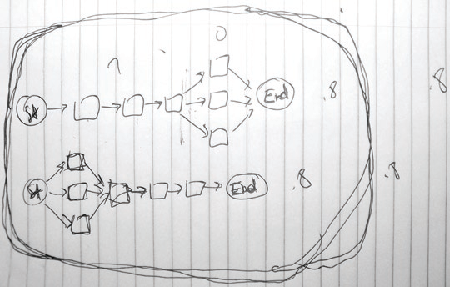
\includegraphics[width=\linewidth]{img/sketch-type-project-management.pdf}
    \caption{Project management diagram showing task precedence of two
      projects. Hastily drawn boxes and arrows represent abstract
      activities.}
    \label{fig:sketch-type-pm}
  \end{subfigure}
  \hspace{1cm}
  \begin{subfigure}[b]{0.42\textwidth}
    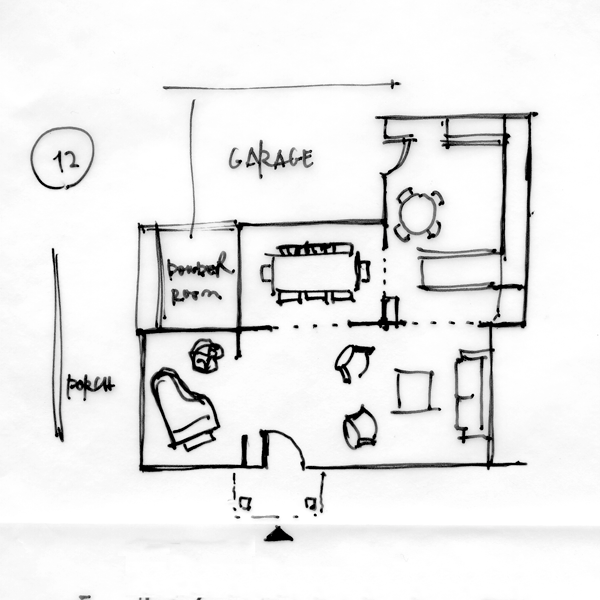
\includegraphics[width=\linewidth]{img/sketch-type-architecture.pdf}
    \caption{An architect's floor plan sketch. It includes text, 
      spatial information, and symbols representing household
      items like a piano or dining table.}
    \label{fig:sketch-type-architecture}
  \end{subfigure}
  
  \caption[Project Management and Architecture Sketches]{Sketches vary
    in domain and in the visual characteristics of marks.}
  \label{fig:types-of-sketches}

\end{figure}


While designing, we iteratively explore and refine the problem
definition and proposed solutions. Sketching supports this creative
search process. We set out on our design task with some high-level
goals. However, due to the
ill-structured~\cite{simon-ill-structured-problems} and ``wicked''
nature of design~\cite{rittel-wicked}, we encounter unforeseen
opportunities and constraints as designing progresses. Those
opportunities and constraints may be implicit in the original problem
description, but designers expose them as they explore. The
discoveries are incorporated into the understanding of the problem and
potential solutions. Design problems are ``not the sort of problems or
puzzles that provide all the necessary and sufficient information for
their solution~\cite{cross-nature-nurture}.'' So it goes with
sketching. We draw different views of our model, which allows us to
perceive the problem in new ways.

Designers engage in a sort of ``conversation'' with their sketches in
a tight cycle of drawing, understanding, and
interpreting~\cite{schon-kinds-of-seeing}. Goldschmidt describes this
as switching between two reasoning modes: ``seeing that'' and ``seeing
as''~\cite{goldschmidt-dialectics}. Seeing \textit{that} is the
process of recognizing the literal, descriptive properties of the
drawing.  Seeing \textit{as} is figurative and transformative,
allowing the designer to re-interpret parts of the sketch in different
ways. Care must be taken to support this conversation when developing
sketch based modeling tools. If the system interprets drawings too
aggressively or at the wrong time, it may prevent the human designer
from seeing alternative meanings; recognize too little and the
software is no better than paper.

\subsection{Prototyping and fidelity}
\label{sec:traditional-prototyping}

Newman and Landay's ethnographies of web designers focused how
designers use informal techniques~\cite{newman-web-designers}. They
found that designers always sketch at the beginning of a web design
project, exploring numerous high-level options. Frequently this early
sketching phase is accompanied with construction of low-fidelity
prototypes made on paper or with Microsoft PowerPoint. As the design
progresses and designers begin incrementally adding details, they move
to higher fidelity models. Client meetings are an important forcing
function in web design projects. When meeting with clients, designers
want to show polished prototypes produced with computer
software. Therefore designers used electronic tools earlier in the
process than they would otherwise have preferred.

Today most software tools support incremental refinement and
specification of details but do not adequately support idea generation
or exploration~\cite{terry-creative-ui}. Designers who begin using
software tools in the early phases of design tend to make superficial
explorations of possible solutions. Further, because tools are poor
for exploration but good for specifying details (font, line weight,
and color), designers tend to focus on nuances that are not yet
important. Observing that current tools are inadequate for creative
pursuits, researchers have developed calligraphic tools such as SILK
and DENIM, which aim to support the early phases of
design~\cite{landay-silk,lin-denim}.

Paper sketches dominate the early phases of design as people generate
new ideas, in a process Goel terms ``lateral
transformations''~\cite{goel-sketches-of-thought}. But as soon as the
web designer believes he or she will make incremental revisions (which
Goel calls ``vertical transformations'') they switch to a computer
tool.

\section{Sketches as a symbol system}

% Cartoon clouds or trees: Overloaded, Ambiguous
\begin{figure}
  \centering
  \begin{subfigure}[b]{0.3\textwidth}
    \centering
    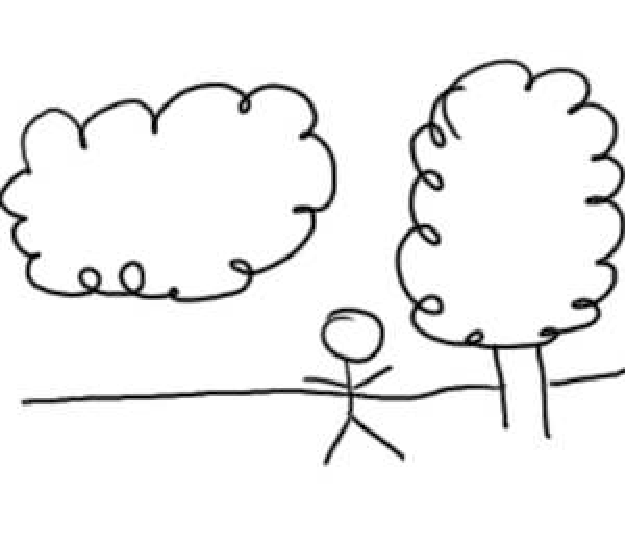
\includegraphics[width=\textwidth]{img/cloud-1.pdf}  
    \caption{Overloaded semantics: The cloud and tree have similar
             shapes but different meanings due to context.}
    \label{fig:cloud-1} 
  \end{subfigure}
  \hspace{0.03\linewidth}
  \begin{subfigure}[b]{0.3\textwidth}
    \centering
    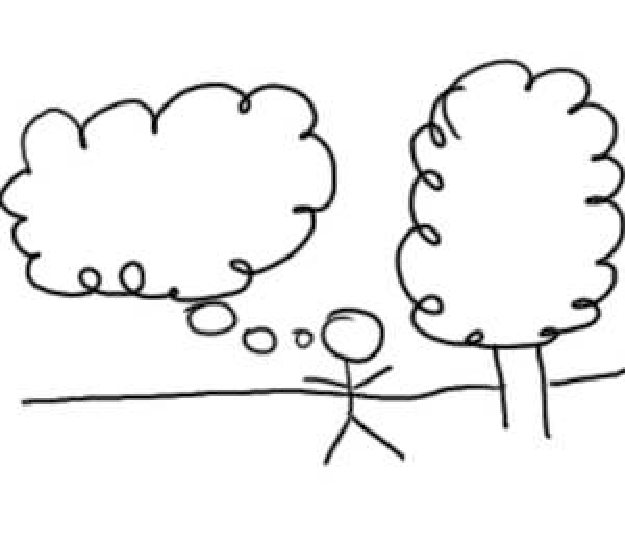
\includegraphics[width=\textwidth]{img/cloud-2.pdf}  
    \caption{Ambiguity: A small addition changes our
      interpretation. The object at left may be a cloud or a thought
      bubble.}
    \label{fig:cloud-2} 
  \end{subfigure}
  \hspace{0.03\linewidth}
  \begin{subfigure}[b]{0.3\textwidth}
    \centering
    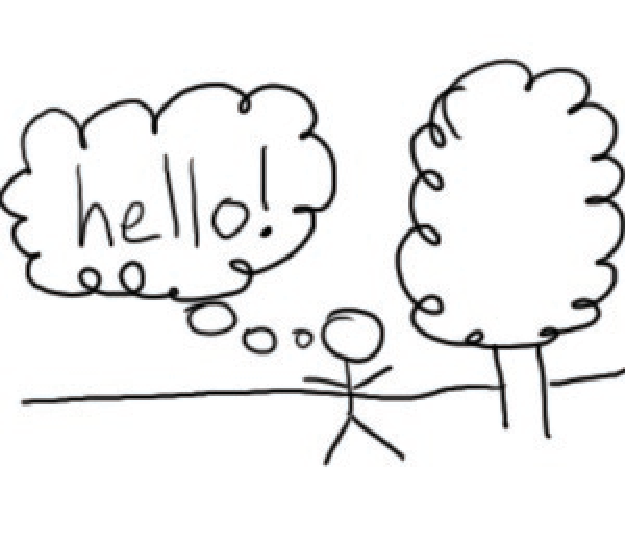
\includegraphics[width=\textwidth]{img/cloud-3.pdf}  
    \caption{More information gives more confidence about object
      identity. Text in the cloud indicates a thought bubble.}
    \label{fig:cloud-3} 
  \end{subfigure}

  \caption[Overloaded semantics and ambiguity]{Overloaded semantics
    and ambiguity.}
  \label{fig:cloud}
\end{figure}


Goodman provides a comprehensive framework for analyzing the
properties of various symbol systems, including
sketches~\cite{goodman-symbols}. Goel places sketching in Goodman's
framework, noting that sketches have \textit{overloaded semantics},
they are \textit{ambiguous}, \textit{dense}, and
\textit{replete}~\cite{goel-sketches-of-thought}. These properties
describe one particular sense of sketching in which the drawer's marks
may be idiosyncratic. It is critical to understand these properties
when developing sketch-based design software.

Sketches have ``overloaded semantics'': The same symbol may mean
different things depending on context. Further, a sketched symbol may
be ``ambiguous'', meaning that the symbol affords more than one
plausible interpretation.  Figure~\ref{fig:cloud} illustrates these
properties. A lumpy shape can be used to indicate many things
including clouds, trees, or thought bubbles. We interpret the shape
differently depending on context.

Sketched symbols are ``dense'', indicating there is a continuous range
between instances of the same symbol. While there may be minute visual
discrepancies between symbol instances, Goel claims that such symbols
are also ``replete'': no aspect of the sketched symbol may be safely
ignored (Figure~\ref{fig:dense-replete}).

The pen strokes constituting a sketch serve various functions. Ink may
indicate abstract domain symbols (e.g. diode, treble clef), object
boundaries, actions (e.g. arrows indicating containment or movement),
dimensions and units, annotations, region texturing, and so on. Some
parts of a sketch are more dense and replete than others. For example
a diode's properties do not change if it is drawn with a slightly
larger triangle. However, subtle variations in how a desk lamp is
drawn might lead to substantially different aesthetic responses to it.

% Stick figures: dense and replete
\begin{figure}
\begin{center}
  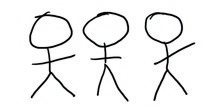
\includegraphics[angle=0, origin=c, width=6cm]{img/dense-replete-stick-figures.pdf}
  \caption[Dense and replete sketches]{Different instances of the same
    stick figure vary along a continuum (\textit{dense}). However, the
    visual properties of individual symbols may (or may not)
    communicate additional information (\textit{replete}). Is the
    figure at the right waving? }

  \label{fig:dense-replete}
\end{center}
\end{figure}


Gross and Do discuss some properties of hand-drawn diagrams from the
perspective of building tools to support design drawing
activities~\cite{gross-ecn-uist}. The authors distinguish sketches
from diagrams, noting that diagrams are ``composed of primitive
elements chosen from a small universe of simple symbols---boxes,
circles, blobs, lines, arrows.'' This list is certainly not
exhaustive, but it does illustrate the general idea that diagrams have
a limited vocabulary. In practice, sketches and diagrams from various
dialects may be combined (e.g. mathematical notation on the same page
as circuit diagrams and hand written notes.)

Freehand diagrammatic drawings are abstract, ambiguous, and
imprecise. \textit{Abstract} symbols denote elements whose identities
or properties are not (yet) important or known. For example,
Figure~\ref{fig:sketch-type-pm} on page \pageref{fig:sketch-type-pm}
shows a project management diagram of two hypothetical projects. The
activities composing each project are abstract---they could represent
anything. The value of the sketch is that it shows the project's
network topology and does not draw attention to what the specific
activities are. 

An \textit{ambiguous} symbol has many plausible interpretations. The
floor plan sketch in Figure~\ref{fig:sketch-type-architecture} shows
several rectangles indicating rooms, furniture, shelves, or
counters. Human observers can confidently disambiguate the intended
meaning of some rectangles, but others remain unclear. The
bottom-right of the sketch shows two armchairs and a sofa with an
ambiguous rectangle in the middle that could plausibly represent
either a rug or a coffee table.

Last, freehand diagrams are \textit{imprecise}. Imprecision allows
designers to work with rough values (e.g. ``about two meters wide'')
and avoid premature commitment. Imprecision also indicates that the
design is by no means final.

The notational properties of sketches make them powerful tools for
supporting visual thinking. Designers may leverage ambiguities in
their sketches to see new meanings, for example. However, these same
properties present challenges for accurate software recognition.

The degree to which a drawing is ambiguous, imprecise, and abstract
varies among instances, and people might interpret them differently. A
rough sketch is useful to designers, especially for brainstorming and
incremental development of ideas. But in order for the sketch to be
transformed into a finished product (e.g. as a digital model supplied
to a rapid manufacturing device), it must be made unequivocal,
precise, and concrete. The process of moving from the informal sketch
to the formal specification involves drawings that are semi-ambiguous,
partially precise, and with some abstractions given definite
identities.

\subsection{Summary: traditional sketching and computation}
\label{ref:traditional-summary}

If we hope to effectively support sketching with computation, we must
first understand the practical aspects of traditional sketching. 

Sketching is an important---perhaps necessary---tool for doing
design. It gives us a way to quickly make provisional drawings, which
help us efficiently make sense of spatial, relational
information. Sketches let us make marks that are as vague or specific
as we need. Because sketched elements can easily be ambiguous, rough
drawings afford different interpretations. We may therefore reflect on
our sketches and see new meaning in existing marks. People sketch in
part because they don't know exactly what they are making---sketching
facilitates exploration.

Low-fidelity prototypes are especially important as tools to test
ideas during early design. This is because they are easy to make,
allowing designers to quickly expose problems before committing to
decisions. Sketching is a common method of creating such prototypes.

In order for computers to recognize sketches, we must develop
techniques to transform imprecisely made marks into discrete
symbols. However, some of the properties that make a sketch useful for
a human (overloaded semantics, ambiguous, imprecise, etc.) complicate
the task of computer recognition.

%% Be sure to also talking about pragmatic vs. epistemic actions, and
%% the tentative, explorational nature of design sketching.

\section{Computational Support for Sketching}

\subsection{Sketching Hardware: Tablets and Pens}

Researchers in sketch recognition and interaction typically use tablet
devices such as a Wacom Bamboo or Cintiq. Some, like the Bamboo,
simply sense stylus input but do not display feedback. These ``blind''
tablets require the user to look at one place (their computer display)
but draw on another surface. This can lead to hand-eye coordination
trouble. The Cintiq, and various Tablet PC computers, combine display
and sensing surfaces. In this case, the user's pen comes into contact
with a drawing plane that is separated from the display plane by only
a few millimeters. When the user views the display at an angle, this
parallax difference can be annoying, but it is certainly better than
the situation with blind tablets.

Input surfaces that are intended to be used with fingers or hands
offer different interaction experiences than pen-oriented drawing
surfaces. For example, users may trace shapes with a single finger,
use two fingers to zoom in or out, or use whole-hand gestures for
issuing other commands. These interaction techniques provide
opportunities for developing innovative sketching applications, as
demonstrated by work by Hinckley \textit{et. al} at Microsoft
Research~\cite{hinckley-pen-touch}.

Regardless of sensing technology, these devices allow users to provide
input in a way that is much closer to handwriting than a mouse
allows. Although pen and mouse input share many properties (both allow
users to interact with 2D displays) they have several key differences.

Mouse input affords \textit{motion} sensing while pen input
affords \textit{position} sensing~\cite{hinckley-input-technology}. In
other words, while mice produce the relative \textit{change} in
$(x,y)$ locations, pens directly provide absolute $(x,y)$ locations.
Users can configure tablets to report relative position, thereby
behaving like a mouse.

Form is also extremely important. A stylus affords people to use the
fine motor abilities of their fingers to control the tip of the pen,
whereas hand and forearm muscles dominate mouse usage. Fingers can be
used to move the mouse, but not with the same dexterity possible with
a pen. Depending on the type of work, a pen may be ergonomically
superior to a mouse, or the other way around.

\begin{figure}
\centering 

\subfigure[Pressing a mouse button exerts force perpendicular to the
  operating plane.] { 
  \label{fig:button-force-mouse} 
  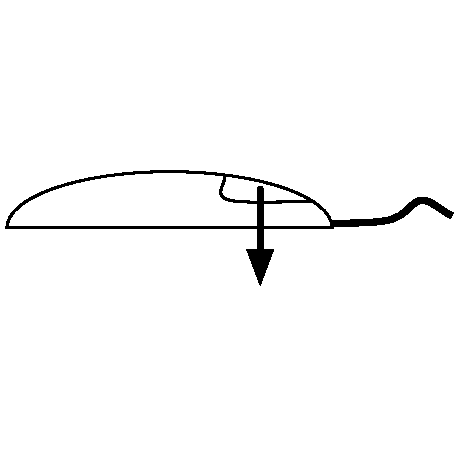
\includegraphics[origin=c, width=5.5cm]{img/button-force-mouse.pdf} 
}
\hspace{1cm} \subfigure[Pressing a stylus button is likely to cause
  accidental pen tip movement.] {
    \label{fig:button-force-pen}
    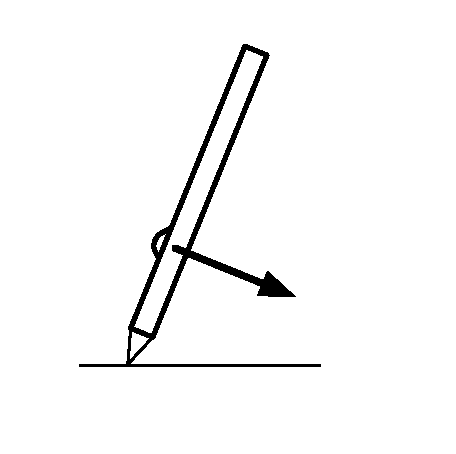
\includegraphics[origin=c, width=5.5cm]{img/button-force-pen.pdf}
}
\caption[Pen vs. Mouse]{The force required to press a mouse button compared with a
  stylus button.}
\label{fig:button-force}
\end{figure}


Some styluses have buttons. While buttons are an indispensable part of
a mouse, they are often difficult to use on the barrel of a
pen~\cite{plimmer-pen-usability}. The force of a \textit{mouse} button
click is orthogonal to the device's plane of use and has negligible
effect on target accuracy. However, pressing buttons on a
\textit{stylus} can move the tip of the pen, making it difficult to
press the button while pointing at particular objects (see
Figure~\ref{fig:button-force}). Further, pressing a button on a
computer stylus usually requires the user to adjust the pen in
hand. This action may be distracting and uncomfortable for long term
use.


%% Distinguish between ``faithful'' and ``faux'' sketching
%% systems. Faithful tools respect the tentativeness of physical
%% sketching where people don't have all the answers at the start. Faux
%% sketching systems are named so because the developers view their tools
%% as being fast, but they do not support sketching as on paper.

%% Within computational support for sketching there are a bunch of
%% technical areas to look at. Can crib a lot from the lit review. The
%% sections that are most important are:

%% \begin{itemize}
%% \item Ink Parsing (corner finding, segmentation)
%% \item Recognition
%% \item Domain modeling
%% \item Graphics (rectification, rendering)
%% \item Interaction techniques, interaction design
%% \end{itemize}

         % trad. design sketching, sketch recog (mini things)., SBIM overview
\chapter{Formative Studies}

\section{Tiny Ethnography}

\section{Interviews}

\section{Artifact Analysis}




  % formative studies: MAYA ethnography, interviews, artifact analysis
\chapter{Sketch It, Make It: Overview}

The primary contribution of this thesis is the set of interaction
techniques implemented in a single design tool called Sketch It, Make
It (SIMI). SIMI is a modeling environment for laser cutter design that
recognizes short sequences of drawn input made with a stylus. Using
only freehand input, SIMI enables a designer to iteratively and
incrementally create precise laser cut models.

I am inspired by the potential of freehand drawing as the basis for
precision modeling for several reasons. Sketching is quick and can be
easily learned. It is simple and modeless: unlike structured editing
software, a designer need not set a pencil's mode to line, circle, or
anything else. I will show that given an appropriate set of
interaction methods, sketched input can provide enough information to
make a precise digital model.

There are several principles that guided SIMI's design and development.

\begin{itemize}
\item \textbf{Democratized design}: Freehand drawing is a skill that
  most people already have. It follows that a tool based on sketch
  based interaction should be usable by a majority of people. For this
  reason I target avocational designers, not professionals. 
\item \textbf{Sketch based}: The user should never feel obliged to set
  down their pen. In the past, many sketch based design tools have
  relied on keyboard input, or used interface widgets that are
  appropriate for mice but are uncomfortable to use with a stylus
  (e.g. hierarchic menus).
\item \textbf{Coherence of interaction techniques is key}: The tool
  presents a set of sketch based interaction techniques that work well
  together. Researchers commonly make toy systems that demonstrate one
  or two novel interaction techniques in isolation (e.g. my own prior
  work on Flow Selection~\cite{johnson-flow-selection}). But a useful
  tool has many individual techniques. The current system implements
  many techniques together to give an example of a way to make them
  work harmoniously.
\item \textbf{Useful and usable}: Last, the system lets people make
  real things in a real domain (namely, laser cut objects). The
  current implementation of the tool is efficient and highly
  responsive. In informal demonstrations, more than one person has
  noted that the system seems more like a commercial product than a
  research system. This is intentional.
\end{itemize}

\section{Rapid Fabrication and Laser Cutting}

Laser cutters are among the more common and affordable fabrication
machines. One can think of a laser cutter as a fast, strong, and
precise automated razor that cuts flat material (paper, wood, plastic,
textiles, etc.). 

% Price information: 
% 2001: 12,900 (ULS 25 watt)
% 2006: 9,995 (ULS 25 watt)
% 2010: 8,500 (ULS 25 watt)
% 2011: 6,850 (ULS 25 watt)
%
%   http://www.rcgroups.com/forums/showthread.php?t=16912 claims that
%   a 25-watt model from Universal Laser systems cost $12,900. Several
%   comments in that thread are in line with that price estimate for
%   home-garage-lab use.
%   http://www.microgeo-usa.com/ProductDetails.asp?ProductCode=universal-laser-VLS2.30
%   currently prices the ULS 25 watt 16x12 unit as costing $6,850.

% http://55-website.com/xo1/ulsinc/english/PDFs/EJ_VL_Article_Reprint.pdf is a press article from 2006 that prices the 25 watt laser at 10,000
\begin{figure}[b] %  figure placement: here, top, bottom, or page
   \centering
   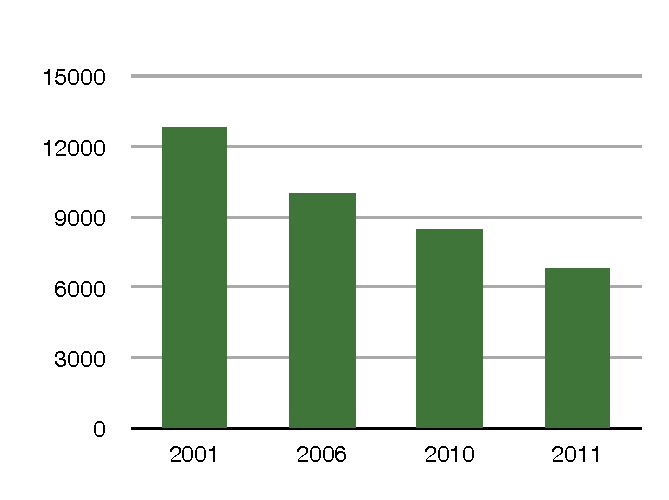
\includegraphics[width=3in]{img/prices.pdf} 
   \caption[Declining laser cutter prices]{Declining prices of Universal Laser Systems 25-Watt 16x12
     inch laser cutter (US Dollars).}
   \label{fig:prices}
\end{figure}


The price of laser cutters is quickly declining, making it possible
that more people have access to them. Figure~\ref{fig:prices} shows
prices for a comparable~25-Watt,~16''x12'' laser cutter model from
Universal Laser Systems (these values were found on hobbyist web
forums). While these data may not be exact, they do show the price of
desktop laser cutting machines has been cut by almost half in the past
ten years. While still out of reach for most people to afford, they
are becoming inexpensive enough for schools and hacker spaces to own.

Laser cut designs are composed of parts cut from solid, flat material
and assembled in various ways: laminated, notched, bolted together,
\textit{etc}. Various materials require different laser speed and
intensity settings to achieve a quality cut. The designe uses a
software application to specify part shapes for laser cutting. The
software outputs vector graphics called a ``cut file'' that defines
these shapes. As most joints have small margins of error, lengths,
angles, and relative position must be specified precisely so that
parts fit together properly.

Tools for designing laser cut objects must allow users to precisely
specify dimensions. Like a physical saw, the laser leaves a gap in its
wake, called a \textit{kerf}, (between 0.2mm and 0.5mm on a 40 watt
cutter). This is an important consideration when designing facets
whose tolerances are small with respect to kerf. A notch joint, for
example, is ineffective if it is 0.1 mm too large or small.


\section{Motivating Scenario: Pictureframe Holder}

\begin{figure}
  \centering
  \begin{subfigure}[b]{0.45\textwidth}
    \centering
    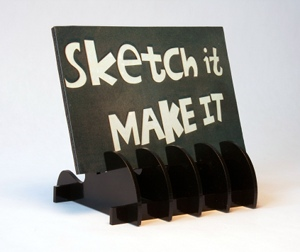
\includegraphics[width=\textwidth]{img/simi-stand-withpic.jpg}
    \caption{} % force the (a) to show up
    \label{fig:example-1}
  \end{subfigure}
  \begin{subfigure}[b]{0.45\textwidth}
    \centering
    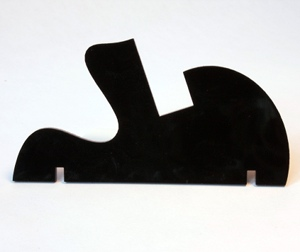
\includegraphics[width=\textwidth]{img/simi-stand-part.jpg}
    \caption{} % force the (b) to show up
    \label{fig:example-2}
  \end{subfigure}
  \caption[Picture Frame Stand]{A picture stand (\subref{fig:example-1})
    drawn and fabricated using SIMI. A single copy of the primary part
    is shown in (\subref{fig:example-2}). }
  \label{fig:simi-example}
\end{figure}


To introduce Sketch It, Make It we show how we use it to make the
picture stand shown in Figure~\ref{fig:simi-example}. We begin with
the idea of a stand with two horizontal rails as a base and a
five-part vertical support structure, joined with notches.

We first draw the rough profile of the vertical support piece using
curved and straight segments. SIMI captures our drawing, straightening
lines, smoothing curves, and connecting curved and straight segments.
 
After sketching the rough outlines of our two parts, we begin to
refine the design and make it precise.  We square the corners by
drawing right-angle braces (Figure~\ref{fig:motivating}a).  Now as we
adjust the shapes of the two parts by selecting and dragging endpoints
and re-shaping curves, SIMI maintains the right-angle constraints
we've established.
 
Next, we add notches to the two parts for the joints. We draw five
small notches on the base rail. For each notch we draw three lines
inside the outline of the part, and then use the erase gesture to
remove the residual outline segment (Figure~\ref{fig:motivating}b).
Then we indicate that both sides of the notch are to be the same
length: We draw tick marks on each segment, and right-angle braces to
keep the notch perpendicular to the edge of the part. The notches must
have exactly the right dimensions: too wide, the top parts will
wobble; too narrow and they will not fit. We size the notch by
overtracing its segments and entering fixed dimensions
(Figure~\ref{fig:motivating}c).
 
We drag the base part (twice) and the support part (five times) to
SIMI's cut file area to prepare a PDF file for cutting, and then send
it to the laser cutter.  Finally we assemble the cut parts to make the
picture stand in Figure~\ref{fig:simi-example}.

\begin{figure}[h]
  \centering
  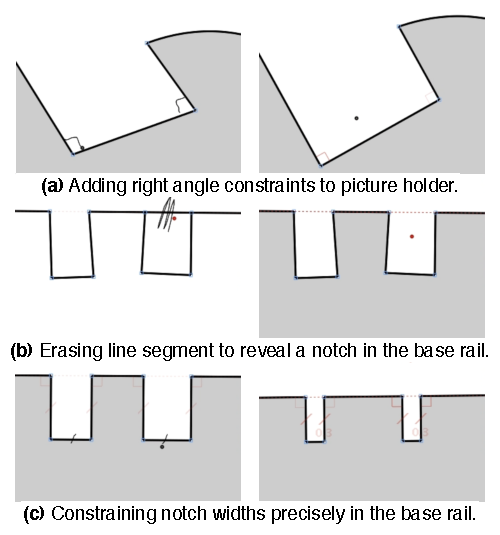
\includegraphics{img/motivating-example.pdf}
  \caption{Key steps taken when making the picture stand.}
  \label{fig:motivating}
\end{figure}


%% The second example is cribbed from the video. It is of the user
%% designing a picture frame holder. It involves:

%% \begin{itemize}
%% \item Using a tablet, most likely a `blind' tablet with separate
%%   display. Introduces hand/eye coordination issues.
%% \item Having the idea in the first place
%% \item Drawing roughly
%% \item Mistakes: errors (the user or the system makes errors) vs. ``on
%%   second thought'' mistakes
%% \item Adding details
%% \item Imagining 3D construction. Admit the tool should support this
%%   directly
%% \item Fabrication: making the cutfile, laser cutting, and assembling
%% \item (maybe) another iteration
%% \end{itemize}

\section{Technical Challenges Met By SIMI}

%% The above section describes the user's needs, and how the user
%% interacts with the system. This section introduces broadly how the
%% system is built to support those needs and interaction. Briefly, the
%% technical aspects are:

%% \begin{itemize}
%% \item Ink parsing (finding corners and segments, removing hooks)
%% \item Recognition (dynamic or post-hoc)
%%   \begin{itemize}
%%   \item Glyphs (akin to character recognition, like right angles)
%%   \item Gesture (recognizes grammatical patterns like erase or
%%     encircle)
%%   \end{itemize}
%% \item Disambiguation of recognized things
%% \item Data model and constraints
%%   \begin{itemize}
%%   \item User sketches things, system reates/maintains constraints
%%   \item Uses iterative, numerical relaxation method
%%   \item Only has X basic constraint types underlying everything
%%   \item High-level ``user constraints'' composed of low-level constraints
%%   \end{itemize}
%% \item Cutfile generation
%%   \begin{itemize}
%%   \item Basic typewriter algorithm. nothing fancy
%%   \item Scales things appropriately
%%   \item PDF output for Illustrator, SVG output for Ponoko (explain why
%%     format matters)
%%   \end{itemize}
%% \end{itemize}

%% From the user's perspective, SIMI gives a new kind of experience
%% because it:

%% \begin{itemize}
%% \item Is ``modeless''. Should describe the mode problem, why
%%   overcoming it is such an important thing, and why it is especially
%%   pertinent to sketch-based interaction. (because if we have modes, we
%%   are essentially on slippery-slope to MouseCAD)
%% \item Is incremental, rather than one-big-batch style recognition that
%%   is so popular
%% \item Uses ``more natural'' input. The pen is easier to manipulate
%%   than the mouse. Naturalness is a common term but is ultimately
%%   meaningless because all design tools are artificial. Could say it
%%   has less cognitive and ergonomic demands than modal, mouse-based
%%   tools
%% \item From a domain perspective it is not over featured, so it is
%%   clear how to proceed.
%% \end{itemize}
   % rapid fab, laser cutting, 'the process', introduce SIMI from high level
\chapter{Sketch It, Make It: Details}

The previous chapter gave an overview of SIMI's architecture. This
included an introduction of SIMI's recognition process.
(Section~\ref{sec:recognition-architecture}). This chapter gives
details on how each recognizer works. 

First, SIMI's corner finding and segmentation strategy is
described. This process is necessary to most recognition, and is what
produces geometric output like lines and arcs. Next, the three types
of recognizers are described: including Dynamic, Pen Up, and Delayed
recognizers. All sketch based interaction techniques are detailed in
these sections.

\section{Ink Parsing}
\label{sec:corner-finder}

Ink parsing is the process of identifying useful characteristics of
raw ink, such as the locations of corners, curvature at specific
points, and the likely identities of segments like lines or curves.

In the following sections, there are two different ways to measure
distance: Euclidean and Curvilinear (see
Figure~\ref{fig:distance-measures}). Euclidean distance is the
measurement most people are familiar with: this is how far apart two
points are on the 2D plane. Curvilinear distance follows the ink
stroke path. In the figure, points A and B are close together in the
Euclidean sense, but are farther apart in the Curvilinear sense. The
Euclidean and Curvilinear midpoints are also depicted in
Figure~\ref{fig:distance-measures}. 

\begin{SCfigure}%[t]
  \centering
  \caption[Euclidean vs. Curvilinear Distance]{Two ways to measure
    distance: Euclidean vs. Curvilinear. The Euclidean distance from A
    to B is direct ($length=18$). Curvilinear distance from A to B
    follows the path indicated ($length=86$). Each measurement
    approach has a related midpoint, indicated as smaller dots.}
  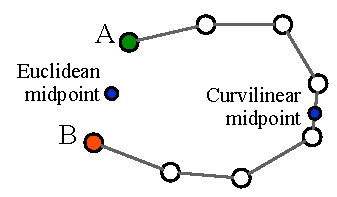
\includegraphics[width=3in]{img/distance-measures.pdf}
  \label{fig:distance-measures}
\end{SCfigure}


SIMI's ink parsing strategy is simpler than many other approches from
the SBIM literature. Others, like the strategies taken by
Sezgin~\cite{sezgin-early-processing} or Wolin~\cite{wolin-smr},
combine both \textit{time} and \textit{curvature} information when
corner finding. SIMI's approach relies only on curvature, but still
achieves good results.

When the user completes a stroke, the ink parser is invoked. First it
assigns a curvature value to each point. Next, a corner finder uses
this data to identify which (if any) points along the stroke are
corners. Last, the system analyzes the regions between corners to
determine the most likely segment type. The output of this process is
the set of segmets formed in the last step. I will detail each of
these steps now.

\subsection{Curvature}

\begin{figure}
  \centering
  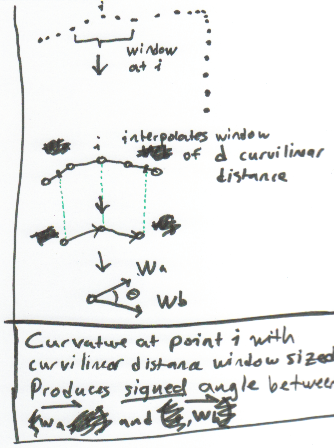
\includegraphics[width=2in]{img/curve-diagram.png}
  \caption[Curvature]{Illustration of how SIMI computes curvature about point $p_i$.}
  \label{fig:curvature-diagram}
\end{figure}


Figure~\ref{fig:curvature-diagram} illustrates how curvature is
calculated. A rough ink stroke has a series of points that are not
evenly spaced out. Sometimes, they may be very close together (for
example, when the user draws slowly). To determine the curvature at an
individual point, we must look at a nearby region called a
\textit{window}, rather than the immediate neighbors. Without this
window, the curvature would be unreliable when points are very close
together.

The window's size $w$ is determined by the current zoom factor. When
the zoom factor is 1 (meaning there is a 1:1 ratio between model and
screen coordinates), the window size is 20 (corresponding to 20
pixels). To calculate the window boundaries at point $p_i$, the corner
finder begins at $p_i$ and traverses the stroke backwards and forwards
by half the window size. It computes interpolated points $w_a$ and
$w_b$ that are exactly $w/2$ units along the stroke to $p_i$. It then
forms two vectors: $v_a$ from $w_a$ to $p_i$, and $v_b$ from $p_i$ to
$w_b$.

The signed curvature $\theta$ for $p_i$ is computed directly from
these two vectors. The magnitude is determined by their dot product;
the sign is determined by the cross product.

\begin{samepage}
\begin{equation}
  \theta_{unsigned} = \arccos \frac{v_a\cdot v_b}{|v_a| |v_b|}
\end{equation}

\begin{equation}
  \theta = \left\{ 
  \begin{array}{r l}
    \theta_{unsigned} & \quad \text{if } |v_a \times v_b| \geq 0\text{,}\\
    -\theta_{unsigned} & \quad \text{otherwise}\\
  \end{array} \right\}
\end{equation}
\begin{samepage}

It is tempting to use $\arctan$ to calculate curvature because it is a
simple calculation. However, this leads to discontinuities when the
vertical change is zero. The approach described above is valid for any
orientation.

\subsection{Isolate Corners}

Now that each point's curvature has been calculated, we can identify
corners. This is a two-step process illustrated
in~Figure~\ref{fig:corner-finding}. First, clusters of high curvature
are identified. To be a member of such a cluster, the absolute value
of a point's curvature must be greater than some threshold. In the
current version of SIMI this value is 45 degrees.

\begin{figure}
  \centering
  \begin{subfigure}[t]{0.4\textwidth}
    \centering
    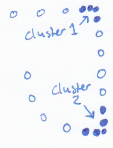
\includegraphics[width=1in]{img/corner-clusters.png}
    \caption{Clusters of high curvature.}
    \label{fig:corner-clusters}
  \end{subfigure}
  \hspace{1cm} % spacing, do what you need
  \begin{subfigure}[t]{0.4\textwidth}
    \centering
    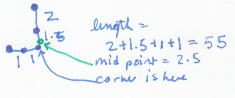
\includegraphics[width=2in]{img/corner-isolation.png}
    \caption{Corner point is closest to middle of cluster.}
    \label{fig:corner-isolation}
  \end{subfigure}
  \caption[Corner finding]{Corner finding involves clustering nearby
    points with high curvature, and choosing the point closest to the
    curvilinear middle of each cluster.}
  \label{fig:corner-finding}
\end{figure}


Once clusters have been computed, a corner is found for each. A
cluster's corner is simply the point closest to the curvilinear
middle. In other words, if the distance along stroke from the
beginning to the end of the cluster is 9, the corner is the point in
the cluster that is nearest to the interpolated point 4.5 units from
the cluster beginning. 

In addition to the corners discoved in this process, the stroke's
first and last points are also included as `corners'. This is for the
convenience of the next step where segments are identified.

\subsection{Identify Segment Types}

The last step in ink parsing is to identify segment
types. Table~\ref{tab:segment-types} in the previous chapter describes
the possible segment types. For each segment type there is a
corresponding segment finder. The segment finders for `open' types
(Line, Arc, Spline) operate on regions between corners. The remaining
segment finders are identified by examining the raw ink directly, and
do not use corner data.

Like semantic sketch recognizers, it is possible for multiple segment
finders to positivly identify ink. To mitigate this, segment finders
operate on a priority system. The priority is: Dot, Circle, Ellipse,
Blob, Line, Arc, and Spline. In other words, if the Dot finder
identifies a dot, there is no possibility of the associated ink being
identified as a Circle.

\subsubsection{Dot Finder}

The dot finder examines the entire ink stroke. If the entire stroke
was made in less than some threshold value (currently 180
milliseconds), it is always considered a dot. Otherwise, it continues
by computing the convex hull of all stroke points. Two properties of
the hull are used next: the area and the aspect ratio. If the ratio
defined by $ratio = area/aspect$ is less than 120, it is a dot. If
not, there is one final check to make. The stroke's point density is
computed. This is the number of points in the original ink stroke,
divided by the hull's area. If $ratio/(0.3 + density)$ is less than
120, it is a dot.

%% The thresholds used in this section (and many others) were determined
%% by trial and error. Some (such as point density) might need to be
%% changed dramatically if different hardware is used. For example, these
%% numbers were found using a default mouse driver, which reports only
%% integer positions. Ink strokes will be less dense than if a proper
%% tablet driver reports floating point locations.

\subsubsection{Circle and Ellipse Finder}

Circles, Ellipses, and (in the next part) Blobs are the three
\textit{closed} segment types. A segment is closed if the begining and
end points are close, relative to the overall length of the
stroke. More formally given start and end points $p_{start}$ and
$p_{end}$:

\begin{equation}
\begin{array}{rcl}
closeness &
= &
\dfrac{EuclidianDistance(p_{start}, p_{end})}{CurvilinearDistance(p_{start}, p_{end})} &
\\
closed &
= &
\left\{ 
  \begin{array}{r l}
    true & \quad \text{if } closeness \leq .1\text{,}\\
    false & \quad \text{otherwise}\\
  \end{array} \right\} \\
\end{array}
\end{equation}

Circles and Ellipses are identified with the same finder. If the input
stroke is closed, the input is fit to an ellipse. To avoid placing
restrictions on how users can draw, user may draw ellipses at
arbitrary angles. SIMI implements a least squares approach described
by Fitzgibbon \textit{et. al}~\cite{fitzgibbon-ellipse-fitting}. It is
an efficient algorithm whose complexity grows linearly with the size
of the input. The output of the ellipse fitting algorithm is a rotated
ellipse, defined by a centroid, a rotation, and major and minor axis
magnitudes.

An error value is calculated to determine how closely the raw input
matches the derived ellipse. This is done in a modified \textit{least
  squares} fashion that requires the calculating the minimum distance
between a point and the ellipse. Unfortunately this is an involved
process (for example, see ~\cite{eberly-point-to-ellipse}). SIMI
approximates the shortest distance between a point $p$ and an ellipse
by discretizing the ellipse boundary into a list of points $d$, and
computes the minimum distance between $p$ and $d$.

The error value measuring the closeness between raw input points $p_i,
i \in [0..n)$ and the discretized elliptical surface $D$ is given with
  the equation:

\begin{equation}
Elliptical\:Error = \frac{
\sqrt{
\sum min^2(p_i, D)
}
}{
n-2
}
\end{equation}

In order for the input to be considered a Circle or Ellipse, the total
error must be less than 1.0. This value was determined experimentally,
given a discretization of 60 points. To distinguish between a Circle
and an Ellipse, the fit ellipse's eccentricity used. Eccentricity
describes how flattned the ellipse is is defined in terms of its major
and minor radii:

\begin{equation}
Eccentricity = \sqrt{\dfrac{major^2-minor^2}{major^2}}
\end{equation}

If the eccentricity is less than 0.7, the input is a Circle; otherwise
it is an Ellipse.

\subsubsection{Blob Finder}

\subsubsection{Line Finder}

\subsubsection{Arc Finder}

\subsubsection{Spline Finder}

\section{Dynamic Recognizers}

\subsection{Erase}

What is it for? State obvious use quickly, and give detail on any
non-obvious uses.

Recognition process: What kind of data does it use? What is the
context-free recognition like? What context does it use?

What (if any) visual feedback is there?

What actions are taken if it is positively recognized and not
filtered?

Wrote this somewhere else: For example, the Erase gesture went through
a number of design iterations. Each version was only slightly better
than the last, and users were only able to successfully execute the
scribble gesture about half the time. When it failed, the scribble
would be interpreted as linework, which would then require users to
erase that. I then completely changed the erase gesture recognizer so
it would operate as the pen was down. When it found a scribble, a
colored 'X' appeared over the scribble to indicate that the user's
erasure will succeed. This lets users scribble until an X appears,
giving them confidence the system has understood. This reduced the
number of recognition errors substantially.

\subsection{Undo and Redo}

What is it for? State obvious use quickly, and give detail on any
non-obvious uses.

Recognition process: What kind of data does it use? What is the
context-free recognition like? What context does it use?

What (if any) visual feedback is there?

What actions are taken if it is positively recognized and not
filtered?

\subsection{Flow selection}

What is it for? State obvious use quickly, and give detail on any
non-obvious uses.

Recognition process: What kind of data does it use? What is the
context-free recognition like? What context does it use?

What (if any) visual feedback is there?

What actions are taken if it is positively recognized and not
filtered?

\section{Pen Up Recognizers}

\begin{itemize}
\item Remove hooks
\item Get structured ink related to unprocessed ink.
\item Add all new structured ink to the model
\item Apply post-hoc recognizers to new structured ink
\item Disambiguate any conflicting results using (a) context in the
  model and (b) preset rules like right-angle wins over same-length
  (filterRecognizedItems())
\item Apply remaining recognized items. This removes the related
  structured ink from the model.
\item Auto-latch remaining segments with each other and existing model
  segments.
\item Search for cutouts (don't call them stencils anymore)
\item Wake up constraint solver
\item Request state snapshot
\end{itemize}

\subsection{Latching}

What is it for? State obvious use quickly, and give detail on any
non-obvious uses.

Recognition process: What kind of data does it use? What is the
context-free recognition like? What context does it use?

What (if any) visual feedback is there?

What actions are taken if it is positively recognized and not
filtered?

Four kinds: automatic, endpoint, continuation, and t-junction.

\subsection{Pan and Zoom}

What is it for? State obvious use quickly, and give detail on any
non-obvious uses.

Recognition process: What kind of data does it use? What is the
context-free recognition like? What context does it use?

What (if any) visual feedback is there?

What actions are taken if it is positively recognized and not
filtered?

\subsection{Select point}

What is it for? State obvious use quickly, and give detail on any
non-obvious uses.

Recognition process: What kind of data does it use? What is the
context-free recognition like? What context does it use?

What (if any) visual feedback is there?

What actions are taken if it is positively recognized and not
filtered?

\section{Delayed Recognizers}

\subsection{Same length}

What is it for? State obvious use quickly, and give detail on any
non-obvious uses.

Recognition process: What kind of data does it use? What is the
context-free recognition like? What context does it use?

What (if any) visual feedback is there?

What actions are taken if it is positively recognized and not
filtered?

\subsection{Specific length}

What is it for? State obvious use quickly, and give detail on any
non-obvious uses.

Recognition process: What kind of data does it use? What is the
context-free recognition like? What context does it use?

What (if any) visual feedback is there?

What actions are taken if it is positively recognized and not
filtered?

\subsection{Right angle}

What is it for? State obvious use quickly, and give detail on any
non-obvious uses.

Recognition process: What kind of data does it use? What is the
context-free recognition like? What context does it use?

What (if any) visual feedback is there?

What actions are taken if it is positively recognized and not
filtered?

\subsection{Same angle}

What is it for? State obvious use quickly, and give detail on any
non-obvious uses.

Recognition process: What kind of data does it use? What is the
context-free recognition like? What context does it use?

What (if any) visual feedback is there?

What actions are taken if it is positively recognized and not
filtered?
    % N techniques: linework, erase, right angle, pan/zoom, etc.
\chapter{Summative Evaluation}

I evaluated Sketch It, Make It in two ways. First, I tested SIMI
with 60 undergraduate architecture students. The objective was to test
if (and how well) SIMI's sketch-based interaction could be used to
make precisely-defined designs for fabrication. Second, a task-tool
analysis compares the strategy of an experienced SIMI user (me) for
making an object with that of an experienced Illustrator user. This
was done to compare how these starkly different tools require
designers to work.

\begin{figure}
  \centering
  \begin{subfigure}[t]{0.6\textwidth}
    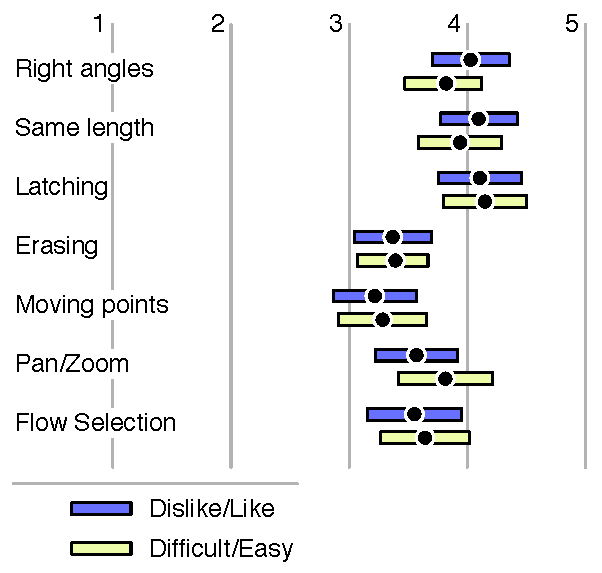
\includegraphics[width=\linewidth]{img/feature-attitude-and-ease.pdf}
    \caption{Questions about features: attitude and ease of use.}
    \label{fig:survey-feature-ease-attitude}
  \end{subfigure}
  \\
  \vspace{5mm}
  \begin{subfigure}[t]{0.8\textwidth}
    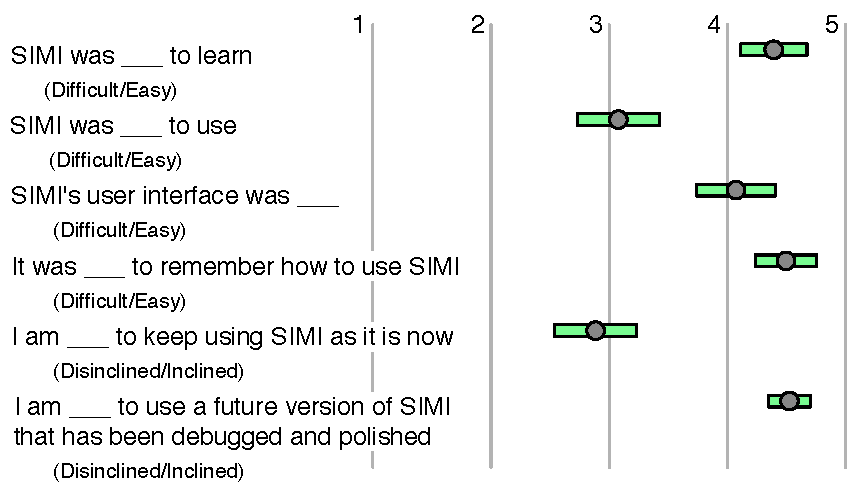
\includegraphics[width=\linewidth]{img/program-attitude-2.pdf}
    \caption{Questions on the system as a whole.}
    \label{fig:survey-program-attitude}
  \end{subfigure}
  \caption[Workshop Survey Results]{Survey results from the workshop
    with undergraduate architecture students. 40 students responded to
    the questionnaire.}
  \label{fig:survey}
\end{figure}


\section{Workshop}

I held a workshop with 60 undergraduate architecture students to
gather qualitative feedback about how easy or difficult SIMI is to
learn and use. The workshop was held in 30-minute sessions over two
days in a room equipped with iMacs and Wacom Intuos
tablets. Regrettably, these tablets do not display output, so users'
eyes are not focused on the same physical location as the pen
tip---leading to significant hand-eye coordination challenges. More
costly display tablets like the Cintiq (Figure~\ref{fig:simi-intro})
avoid this problem, but were unavailable for the workshop.

Initially, students complained that the tablet hardware was difficult
to use, but most of the tablet-related trouble went away after about
ten minutes. Then they quickly learned to make line work and
constraints. At first they had trouble erasing and selecting points,
but soon learned to make these gestures.

I expected students to have difficulty using SIMI because the hardware
(tablets) and interaction paradigm (sketch-based modeling) were both
new to them. However, by the second day, most questions and comments
regarded missing features, not about how to use the system.

After the workshop, students were offered an extra credit assignment
to complete a short survey. This generated 40 responses, summarized in
Figure~\ref{fig:survey}. The survey had three sets of questions, all
on a 5-point scale. The first set asked how easy (or hard) each
interaction method was to use. The second set of questions measured
the student's attitude about the techniques. This line of questioning
was borrowed from~\cite{bae-everybody}.

Only the Erase and point selection gestures seemed to give
participants trouble. These are the only gestures that depend on
timing. Erasing must be done with a quick, vigorous shake of the
pen. Selecting points must be done quickly, or SIMI will interpret the
input as the beginning of a flow selection.

The last set of questions polled students about their perception of
the program as a whole: e.g. how easy it was to learn, to use, and
remember. Although the students reported the system was easy to
\textit{learn}, their responses indicate they found it difficult to
\textit{use}. This might be explained by the limited time available
(one hour), and the novelty of the hardware.

Finally, we asked (1) how much people would like to continue using the
system as it is currently, and (2) how likely they would be to try it
again when it was debugged and nicely tuned. The responses are in
stark contrast: most would not continue using SIMI as it is today,
owing to bugs and lack of features. Despite this, the response to the
second question was very positive.

Enthusiasm about the interaction paradigm of sketching was evident in
comments by respondents. For example:

\begin{itemize}
\item ``This is the start of a great program, and once it is polished it
  will be extremely useful.''
\item ``The program seems like it could be really cool to use in the
  future. I really enjoyed using a tablet and stylus. It made
  designing fun.''
\end{itemize}

Not all commentary was positive. Aside from complaints about bugs,
most negative comments concerned missing features (for example, a
constraint to make lines parallel).

\section{Task-Tool Analysis}

A second method to evaluate our system is to compare the actions
required to make an object with SIMI compared with those of a
conventional tool such as Illustrator.

We asked an expert Adobe Illustrator user to verbally describe the
sequence of discrete actions necessary to model the parts of the table
shown in Figure~\ref{fig:table}. This designer has used Illustrator to
make dozens of laser-cut items.

\begin{samepage}
For example, the first three actions were:

\begin{enumerate}
\item Press the M key to enter rectangle drawing mode.
\item Type rectangle dimensions.
\item Place the rectangle on the drawing canvas.
\end{enumerate}
\end{samepage}

The first action is a persistent mode change, while the second two
specify values. A similar transcript was recorded for SIMI. Five
categories were used to code the verbal protocol. They are listed in
Table~\ref{tab:task-tool-protocol}.


\begin{table}%[h] % [h]ere [t]op [b]ottom [p]age
\centering
\begin{tabular}{l | p{11cm}}
\textbf{Action Type} & \textbf{Description} \\
\hline
&\\

Persistent mode change & 

Change the tool input state so subsequent input is interpreted in
context of that tool (e.g. line drawing mode). User must enter another
persistent mode to exit the first.

\\

Specify value &

Specify a dimension or location.

\\

Specify target &

Indicate (select) an element for a subsequent operation.

\\

Transformation &

Apply an operation that changes existing model elements beyond simply
specifying numeric values. Transformations include moving or erase
items.

\\

Transient mode change &

Temporarily change the tool mode so input is interpreted
differently. This kind of mode change is part of a phrase, and will
revert to another mode when the phrase is complete.

\\
\hline
\end{tabular}
\caption[Task-Tool Protocol Analysis Categories]{Action types used in the task-tool protocol analysis.}
\label{tab:task-tool-protocol}
\end{table}


\begin{figure}[h]
  \centering
  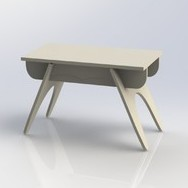
\includegraphics[width=0.4\linewidth]{img/table.jpg}
  \caption[Laser-cut Table Sold on Ponoko]{A laser-cut table for sale
    on Ponoko. We asked expert designers how they would replicate this
    object using either Illustrator or SIMI.}
  \label{fig:table}
\end{figure}

\begin{table}[h]
  \centering
  \begin{tabular}{ l c c }
    \textbf{Action type} & \textbf{Illustrator} & \textbf{SIMI} \\
    \hline
    Persistent mode change & 12 & 0 \\
    Specify value & 17 & 7 \\
    Specify target & 7 & 4 \\
    Transformation & 6 & 27 \\
    Transient mode change & 2 & 0 \\
    \hline
    & \textbf{44} & \textbf{38} \\
  \end{tabular}
  \caption[Action type frequency]{Frequency of action types in the
    design protocol of expert Adobe Illustrator and SIMI users. }
  \label{tab:expert}
\end{table}

The action frequency (listed in Table~\ref{tab:expert}) shows how the
two tools are used to create the same output. Roughly the same number
of actions was taken (Illustrator:~44, SIMI:~38).

To make an object using Illustrator, an expert issues a series of
\textit{Select, Specify} actions: either activate a persistent tool
(e.g. line mode) or select a modeling element (e.g. a line on the
screen), then specify a value or position by typing a number or moving
the mouse.

In contrast, most discrete actions with SIMI involve transforming
geometry that is already on the screen, for example, constraining two
existing lines to meet at a common point or form a right angle. A
single sketched gesture fluidly performs both \textit{Select} and
\textit{Specify} operations that require two distinct actions in
Illustrator. For example, right angle gesture necessarily indicates
the line segments to be constrained.

 % summative eval: 60 undergrads, task-tool analysis, informal reactions
\chapter{Conclusion}

Rapid fabrication---3D printing, laser cutting, and many other
processes---can support designers in ways that were not possible even
ten years ago. But to realize this promise, machine access is not
enough. Users need effective and appropriate design tools.

Sketching is often cited as a common and necessary part of the design
process in many domains. Beginning in the early 1960s with
Sutherland's Sketchpad system~\cite{sutherland-sketchpad}, researchers
have developed sketching systems in many areas, like mechanical
engineering~\cite{lipson-correlation}, web site
design~\cite{lin-denim}, and furniture
production~\cite{oh-fab,saul-sketch-chair}. During this time there has
been a great deal of work on sketch recognition and on isolated
sketch-based interaction techniques. But there has been little effort
in exploring how all this fundamental work can be integrated and
presented as a coherent and useful whole to address real-world design.

This thesis explored the role of sketch based interaction techniques
as a basis for rapid fabrication design tools. I bridged the gap
between an academic treatment of sketch-based design and a real-world
useful and usable system. This work has included a literature review
in design and computational support for sketching
(Chapter~\ref{sec:rw} and the survey with my
committee~\cite{johnson-sketch-review}). Chapter~\ref{sec:formative}
explored the domain of design for laser cutting by studying both
artist and the artifact. Last,
Chapters~\ref{sec:overview}~and~\ref{sec:details} detailed my
\textit{Sketch It, Make It} system that provides a solid example of
how a sketch based system can present a set of sketch recognizers and
(most importantly) interaction techniques to enable real people to do
real work in a way that was previously not actualized.

While I have made a prototype that many observers find compelling,
there is still more work to do. It raises interesting ideas about what
else is possible with this form of interaction, and questions remain
unresolved.

In this chapter I discuss how my work with SIMI can serve as a
starting point for further work. First I discuss the rationale for
providing the particular feature set embodied in this software. Next I
discuss the implications SIMI has on several areas of research. Last,
I describe the most obvious next steps that I would like to take.

\section{Justification of Feature Choices}

SIMI includes a set of interaction techniques that let users perform
actions to create, edit, and build precision models for laser
cutting. This particular collection chosen because it (a) provided a
minimal set of features to be useful, (b) it covered a range of
functions and (c) demonstrated a variety of sketch recognition types.

Some traditional software features were intentionally left out. For
example, \textit{Copy and Paste} is nearly ubiquitous in interactive
systems, but it is not found in SIMI. It is often beneficial to
discard long-standing assumptions of what is necessary to explore
alternate ways to proceed. By omitting Copy and Paste, I had to focus
on making it as easy as possible to create geometry and
constraints. It is possible to create a `copy' of geometry using
standard SIMI actions. This helps to keep the application simple.

\section{Implications to Related Areas}

This research has implications to several areas, including rapid
fabrication hardware and surrounding communities, interaction design,
and research on sketch-based interaction and modeling.

\subsection{Rapid Fabrication and Maker Communities}

Laser cutters, 3D printers, CNC mills and so forth are called
\textit{rapid} prototyping machines because they facilitate fast
machine-work. Often, software design tools are the bottleneck in a
designer's work/build process. While experienced professionals might
master the software to use rapid fabrication machines quickly, the
majority of current (and certainly potential) users have not. Sketch
based interaction might be one part of a new kind democratized design
software that lets hobbyists and amateurs design and make with rapid
fabrication machines.

Inexpensive, widely available, and \textit{easy-to-use} rapid
fabrication hardware and software has interesting
consequences. Economically, it suggests a future where people can
simply ``print'' new objects like door knobs as needed---obviously a
topic of concern for hardware stores and manufacturers. Socially, it
gives regular people the ability to play an active role in the design,
function, and production of everyday things---which is concerning to
professional designers and engineers. While it is difficult to
envision a world without hardware stores (or designers and engineers),
desktop design and fabrication will have serious, unpredictable, and
positive consequences.

\subsection{Interaction Design}

Sketch based interaction may be paired with other input paradigms to
achieve unique results that would not be possible in isolation. While
sketching, the user's non-dominant hand is free to perform other
tasks. This can be leveraged to develop new ways to design. 

Touch input is a current topic of importance, with touch-sensitive
devices like tablets and smart phones dominating the consumer
electronics market. Sketching, paired with touch, has recently been
shown to give compelling results~\cite{hinckley-pen-touch}. New
technologies, such as voice recognition or Microsoft's
distance-sensing Kinect, offer additional avenues that might be
appropriate to mix with sketch-based input. Virtual reality
hardware---special glasses that simulate 3D projection, volumetric
displays, \textit{etc.}---could be used to immerse designers in
augmented reality design tools that let people draw anywhere in
physical space~\cite{jung-lightpen}. These topics have been covered to
various degrees, but the sketch interaction component has always been
ad-hoc. This thesis gives a solid example of one way to support such
interaction. Input paradigms that pair sketching with something else
(touch, gesture, VR) have hardly been explored enough to consider them
known topics.

Currently, sketch interaction is limited to devices that explicitly
support pen interaction. But ongoing advances in sensing technology
(e.g. Touch\'e~\cite{sato-touche}) may allow arbitrary surfaces to
accept sketch and touch input. Further, projection and display
technology continues to advance. When every available wall and
tabletop can display graphics and recognize sketch input, that has
serious consequences for the future of interaction and design.

The recognition and resolution architecture from
Chapter~\ref{sec:overview} might be useful to researchers and
developers working on other kinds of recognition-based systems. For
example, multi-touch devices or Kinect-style hand or body recognition
could use the staged approach to simplify the recognition
process. However, because there are multiple contemporaneous sample
points to consider, future developers might have to extend the
architecture discussed here.

Perhaps most importantly, the staged recognition architecture lets
designers interact with computers using easy-to-make gestures that
richly specify \textit{an action}, \textit{to which objects}, and
\textit{in which way}. This seems to reduce users' cognitive load by
removing the need to enter persistent modes or the needs to set up
sequences of atomic operations to achieve a desired
outcome. Additional work on this topic is warranted.

\subsection{Sketch Based Interaction and Modeling}

This thesis claims that SIMI exemplifies sketch-based interaction
techniques that work well together. However, the particular set is
tuned to the laser cutter domain and to the features SIMI
provides. How can future researchers generalize this contribution?

The recognition and resolution architecture from
Section~\ref{sec:recognition-architecture} guides programmers and
interaction designers to develop new techniques and
applications. While a programming structure is helpful, there are
other important aspects to consider when designing new sketching
gestures.

I provide several heuristics for developing sketch-based interaction
techniques in other applications:

\textit{Leverage context}. Gesture syntax can be overloaded by letting
context determine meaning. For example, a circle drawn around two
unlatched end points is semantically different from a circle drawn
around a cutout. Overloading gestures means less work for the
programmer, and fewer gestures for the user to learn and
remember. However, care must be taken to ensure that the contexts are
separate enough that they will not be confused.

\textit{Substantial shape differences improve recognition and user
  experience}. Strive to develop gestures that are substantially
different from one another. It is tempting to create many gestures
that are different in subtle ways because it is easy to program the
related recognizers. However, users will have a difficult time
remembering and executing these subtly different gestures.

\textit{Rely on visual reinforcement and physical metaphors}. SIMI's
right angle constraint appearance echos the gesture used to create
it. When there is not a visual, the gesture should make physical
sense: the circle gesture used to latch points together feels like
tying the points together with a string; the erase gesture is based on
scratching over unwanted marks on physical paper.

\textit{Make use of the staged recognition architecture}. Some
gestures should be acted upon immediately, while others could (or
should) be deferred until later. For dynamic recognizers, effective
visual feedback is critical. While the staged architecture eases
programming, its true purpose is to improve user experience.

\section{Future Work}

The most interesting research leaves more questions than it
answered. Having built a useful and useful system for laser cut
designs, much of the feedback I receive focuses on additional
features. Observers commonly would like to see a tool like SIMI for
some other domain, such as for 3D modeling.

\subsection{Common Feature Requests}

It is likely that Sketch It, Make It (or something like it) will be
made into a commercial product soon. We have accumulated a long list
of feature requests that can serve as a starting point for the next
set of additional features.

Users like the paper-like feel of the tool, and would prefer to have
the ability to add ink that is not recognized. This enables designers
to explore freely, as they would on paper, while still having the
ability to use these unrecognized portions in future work.

Handwriting recognition is another commonly requested feature. This
was intentionally not included in the current prototype because it
would have required a substantial time investment without a
correspondingly substantial pay-out. Handmade numbers and text could
be applied to give dimensions and labels to parts of a drawing.

Users also request additional constraints, for example making two
lines parallel, or making an object appear at the midpoint between two
others. This would allow a wider and richer range of output.

Another feature that would likely make SIMI much more useful is the
ability to assemble 3D constructions from 2D parts. This would let
users see the relationship between the 2D parts they have designed and
the final 3D output. This can be useful, for example, to identify
stylistic or assembly problems before spending time and material on
the laser cutter.

\subsection{Machine Learning Improvements}

SIMI was built on the idea that it is generally better to give users
interaction techniques to state their intentions, rather than using
machine learning routines to deduce what the user wants. However,
there are a number of cases where machine learning could be used to
make the overall user experience better.

Each user has a drawing style that is different from any other. The
differences can be subtle, or might be substantial. In keeping with
the paper-like interface, an intelligent agent could watch the user
draw and learn their particular style and preferences. For example, if
a user consistently fails to make the erase gesture correctly, their
preferred erasure gesture could be learned and applied (without
asking). The user could also teach the system new gestures entirely,
providing new syntax directly.

Sometimes companies or other organizations adopt conventions. These
conventions may be common within that community but not typically
found outside. SIMI could learn these social norms, and understand
when to apply them.

\subsection{Domain Specific Improvements}

Laser cutters and similar machines (water jet, plasma, CNC mills)
share common properties. If the software could account for these
properties, the user could incorporate them into their designs. An
obvious property of laser cutters is the \textit{kerf}---the width of
the cut path. The laser cutter used throughout SIMI's development
typically leaves a kerf of approximately 0.4mm. When designing
press-fit notches for rigid material that is 3mm thick, the kerf size
is a significant concern. If the tool understood that certain geometry
was sensitive to kerf thickness, the software could save the user time
and material costs by making more accurate cuts.

The press-fit notch just mentioned is just one type of
joint. Currently SIMI does not include a concept of joints. If it did,
the user would be able to indicate where joints should exist, between
which parts, what the material properties are---and the software would
take care of the rest.

Using material is another important consideration, both because it
costs money, and because supplies are often limited. For example,
Ponoko sells 15''x15'' squares of acrylic for between \$8 and \$28
depending on thickness. To make more efficient use of material, the
software could perform intelligent cut file layout with a
shape-packing algorithm. If the system knows where a piece of material
has holes, the algorithm could also place new parts on used material,
saving a lot of money.

Assemblies often have a lot of parts, and it can frustrate users when
trying to determine which part goes where. The tool could etch part
numbers (or joint labels) into the material to aid assembly.

\subsection{Beyond Laser Cutting}

In this work, I set out to demonstrate how a set of interaction
techniques designed to be used together to make a useful and usable
system, and show that sketch-based interaction should be taken
seriously, particularly as a paradigm for doing design. To do this I
picked a specific domain---laser cutting---but there are other domains
that would have been appropriate as well. 

3D modeling is an obvious choice. Physical objects are necessarily
three dimensional, and designers often sketch them in
perspective. There are interesting challenges associated with ``3D
sketching'', and many others are working on these research topics.

2D applications will be easier to write based on SIMI's current
implementation. Graphic design applications for illustrations,
diagrams, logos, T-shirt designs, or cartooning are appropriate areas
for SIMI's interaction.

Teachers famously draw on chalk boards or whiteboards to illustrate
concepts in many areas, from physics to mathematics. A sketch-based
education system might be a useful tool for teaching STEM topics at
all levels---primary, secondary, and post-secondary education.

The techniques presented in this dissertation could potentially be used
in any domain that makes use of structured or semi-structured
diagrams. It could be used to think about ideas, generate concepts. Or
it could be a communication tool used to work with others in ongoing
design projects. Or sketch-based design could simply be used as a
fast, efficient method of specifying the designer's intent to create
finished output.

\section{Looking Forward}

Nearly everything in our environment was deliberately designed and
built by a human being. An artifact's users are not often the same
people that designed or built it. The recent introduction and success
of affordable, fast fabrication machinery suggests the gulf between
\textit{designers} and \textit{users} may narrow as desktop
manufacturing lets ordinary people design and build things on their
own. One remaining bottleneck is software: access to fabrication
machinery is not enough. Democratized fabrication requires
democratized design tools: People need design software that is easy to
use and gives the means to express ideas. But for ordinary people,
current CAD software is expensive, hard to learn, and hard to use.

The sketch-based interaction presented in this thesis explicitly
supports design for laser cut items. This is provided as an example of
a (potentially) much larger space of sketch-based modeling tools. Many
other application areas were mentioned above, such as STEM
applications for students, 3D modeling, animation, and business
diagrams. This line of research is important not simply because it
enables users to do one thing marginally better than before. It is
important because it will empower people to design and make many kinds
of things that were previously impossible. This is a powerful idea,
and the consequences are far-reaching.

 % recap all, future for design is good if keyboard/mouse will just die

%\appendix
%\include{appendix}

\backmatter

%\renewcommand{\baselinestretch}{1.0}\normalsize

% By default \bibsection is \chapter*, but we really want this to show
% up in the table of contents and pdf bookmarks.
\renewcommand{\bibsection}{\chapter{\bibname}}
%\newcommand{\bibpreamble}{This text goes between the ``Bibliography''
%  header and the actual list of references}
\bibliographystyle{plainnat}
\bibliography{sketch-bibliography} %your bib file

\end{document}
